\documentclass[11pt]{article}
\usepackage[utf8x]{inputenc}
\usepackage{polski}
\usepackage{amsthm}
\usepackage{listings}
\usepackage{amsmath}
\usepackage{hyperref}
\usepackage{color}
\usepackage{graphicx}
\usepackage[export]{adjustbox}
\usepackage{float}

\definecolor{mygreen}{rgb}{0,0.6,0}
\definecolor{mygray}{rgb}{0.5,0.5,0.5}
\definecolor{mymauve}{rgb}{0.58,0,0.82}

\lstset{ %
  backgroundcolor=\color{white},   % choose the background color; you must add \usepackage{color} or \usepackage{xcolor}
  basicstyle=\footnotesize,        % the size of the fonts that are used for the code
  breakatwhitespace=false,         % sets if automatic breaks should only happen at whitespace
  breaklines=true,                 % sets automatic line breaking
  captionpos=b,                    % sets the caption-position to bottom
  commentstyle=\color{mygreen},    % comment style
  deletekeywords={...},            % if you want to delete keywords from the given language
  escapeinside={\%*}{*)},          % if you want to add LaTeX within your code
  extendedchars=true,              % lets you use non-ASCII characters; for 8-bits encodings only, does not work with UTF-8
  frame=single,                    % adds a frame around the code
  keepspaces=true,                 % keeps spaces in text, useful for keeping indentation of code (possibly needs columns=flexible)
  keywordstyle=\color{blue},       % keyword style
  morekeywords={*,...},            % if you want to add more keywords to the set
  numbers=left,                    % where to put the line-numbers; possible values are (none, left, right)
  numbersep=5pt,                   % how far the line-numbers are from the code
  numberstyle=\tiny\color{mygray}, % the style that is used for the line-numbers
  rulecolor=\color{black},         % if not set, the frame-color may be changed on line-breaks within not-black text (e.g. comments (green here))
  showspaces=false,                % show spaces everywhere adding particular underscores; it overrides 'showstringspaces'
  showstringspaces=false,          % underline spaces within strings only
  showtabs=false,                  % show tabs within strings adding particular underscores
  stepnumber=1,                    % the step between two line-numbers. If it's 1, each line will be numbered
  stringstyle=\color{mymauve},     % string literal style
  tabsize=4,                       % sets default tabsize to 2 spaces
  title=\lstname                   % show the filename of files included with \lstinputlisting; also try caption instead of title
}

\title{\textbf{Sortowania równoległe i sekwencyjne}}
\author{Dorota Kapturkiewicz\\
		Wiktor Kuropatwa\\
		Karol Różycki}
\date{}
\begin{document}

\maketitle

\section{Cel projektu}
Celem poniższego projektu jest porównanie efektywności i czasu działania kilku algorytmów sortowania z różnym stopniem zrównoleglenia.

\section{Zaimplementowane algorytmy}
Projekt zaostał zaimplementowany w języku C++ (w standardzie c++ 11).
Do fragmentów wielowątkowych użyliśmy biblioteki OpenMP. \newline
Dana praca porównuje działania następujących algorytmów:
\begin{itemize}

\item merge sort 
\begin{itemize}
\item w pełni sekwencyjny 
\item równoległe wywołania rekurencyjne sortowania, sekwencyjne złączanie
\item równoległe sortowanie i złączanie
\end{itemize}

\item bitonic sort
\begin{itemize}
\item w pełni sekwencyjny 
\item zrównoleglone wywołania rekurencyjne i porównywanie wartości w bitonic merge'u
\end{itemize}

\item radix sort
\begin{itemize}
\item w pełni sekwencyjny 
\item zrównoleglony prefix sum, przepisywanie wartości i przygotowywanie danych (xor)
\end{itemize}

\end{itemize}


\section{Przeprowadzone testy}
\begin{figure}[H]
\raggedleft
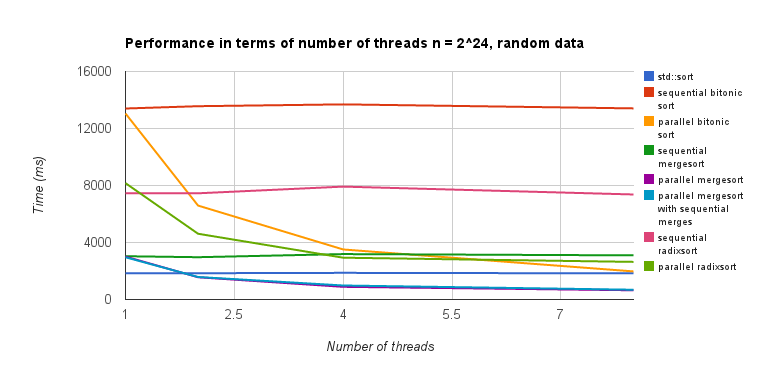
\includegraphics[width=1.20\textwidth, height=0.35\textheight,left]{random_data.png}
\caption{Czas działania w zależności od liczby wątków na losowych danych}
\end{figure}
\begin{figure}[H]
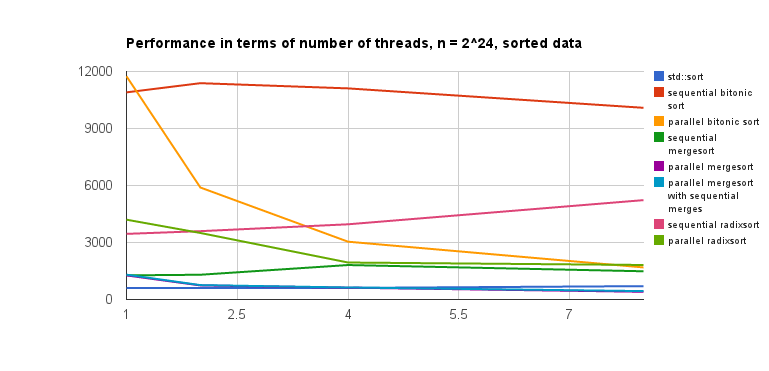
\includegraphics[width=1.20\textwidth, height=0.35\textheight, left]{sorted_data.png}
\caption{Czas działania w zależności od liczby wątków na posortowanych danych}
\end{figure}
\begin{figure}[H]
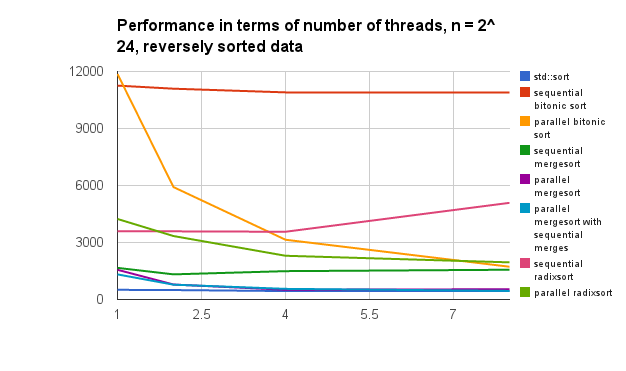
\includegraphics[width=1.20\textwidth, height=0.35\textheight, left]{reversely_sorted_data.png}
\caption{Czas działania w zależności od liczby wątków na odwrotnie posortowanych danych}
\end{figure}
\begin{figure}[H]
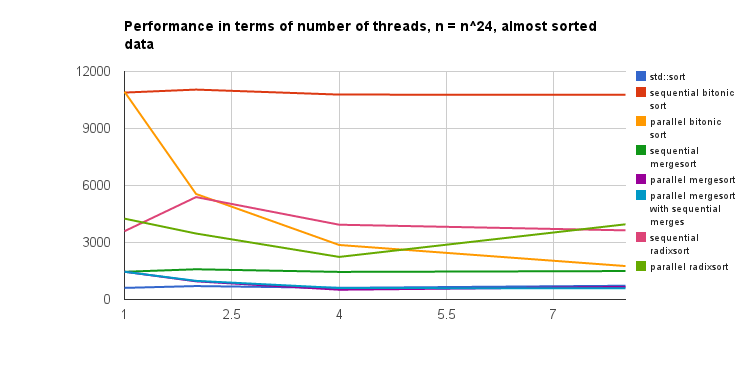
\includegraphics[width=1.20\textwidth, height=0.35\textheight, left]{almost_sorted_data.png}
\caption{Czas działania w zależności od liczby wątków na prawie posortowanych danych}
\end{figure}

\section{Wnioski}
\begin{itemize}
\item
Algorytmy z elementami równoległymi działają lepiej niż sekwencyjne na większej liczbie wątków.
\item
Zrównoleglony mergesort na 2, 4 orazy 8 wątkach działa szybciej niż std::sort. W przypadku pozostałych algorytmów również możemy odnotować znaczacy wzrost wydajności.
\item
Przy użyciu jednego wątku algorytmy równolegle często wykazują gorszy czas działania niż sekwencyjne.
\item
Równoległe bitoniczne sortowanie pomimo gorszej złożoności ($O(nlog^2n)$) jest w stanie wyprzedzić sekwencyjne algorytmy o złożoności $O(nlogn)$.
\item
Ze względu na mała liczbę wątków prefix sum użyty w równoległym algorytmie radixsort nie był w stanie w pełni wykazać swojej mocy, ale i tak możnaby było zauważyć około czterokrotne przyśpieszenie w stosunku do sekwencyjnego.
\item
Równoległy algorytm merge sort okazał się być najszybszym z całej stawki, wyprzedzając nawet algorytm std::sort.
\end{itemize}

\section{Źródła}
Bitonic sort:
\lstinputlisting[language=C++]{bitonic_sort.cpp}

Merge sort:
\lstinputlisting[language=C++]{merge_sort.cpp}

Radix sort:
\lstinputlisting[language=C++]{radix_sort.cpp}


\end{document}
